\documentclass[mathserif,compress,CJKutf8, red]{beamer}

\mode<presentation>
{
  \usetheme{Antibes}
  % 可供选择的主题参见 beameruserguide.pdf, 第 134 页起
  % 无导航条的主题: Bergen, Boadilla, Madrid, Pittsburgh, Rochester;
  % 有树形导航条的主题: Antibes, JuanLesPins, Montpellier;
  % 有目录竖条的主题: Berkeley, PaloAlto, Goettingen, Marburg, Hannover;
  % 有圆点导航条的主题: Berlin, Dresden, Darmstadt, Frankfurt, Singapore, Szeged;
  % 有节与小节导航条的主题: Copenhagen, Luebeck, Malmos, Warsaw

% \setbeamercovered{transparent}
% 如果取消上一行的注解 %, 就会使得被覆盖部分变得透明(依稀可见)
}

\usepackage{CJKutf8}   % 文档使用 UTF8 编码
\usepackage{hyperref}
\usepackage{amsmath,amssymb,amsfonts}
\usepackage{color,xcolor}
\usepackage{graphicx}
\usepackage{manfnt}

\hypersetup{bookmarks=true, % 是否使用书签
                   unicode, % 使用 unicode 编码书签
          colorlinks=false, % 是否使用彩色链接
         pdfborder={0 0 0}, % 链接周围有无边框,{0 0 0}表示无
        pdfstartview=FitBH, % 
    pdfpagemode=FullScreen, % 全屏显示
    pdfauthor={Wenbo Yang}, % pdf 作者
   pdftitle={WSN Security}, % pdf 标题
 pdfsubject={WSN Security}, % pdf 主题
}
\setbeamertemplate{bibliography item}[text]
\setbeamertemplate{blocks}[rounded][shadow=true]

%%%%%%%%%%%%%%%%%%%%%%%%%%%%%%%%%%%%%%%%%%%%%%%%%%%%%%%%%%%%%%%%%%%%%%%%%%%%
%                          定制幻灯片---重定义字体、字号命令                           %
%%%%%%%%%%%%%%%%%%%%%%%%%%%%%%%%%%%%%%%%%%%%%%%%%%%%%%%%%%%%%%%%%%%%%%%%%%%%
\newcommand{\song}{\CJKfamily{song}}    % 宋体   (Windows自带simsun.ttf)
\newcommand{\fs}{\CJKfamily{fs}}        % 仿宋体 (Windows自带simfs.ttf)
\newcommand{\kai}{\CJKfamily{kai}}      % 楷体   (Windows自带simkai.ttf)
\newcommand{\hei}{\CJKfamily{hei}}      % 黑体   (Windows自带simhei.ttf)
\newcommand{\li}{\CJKfamily{li}}        % 隶书   (Windows自带simli.ttf)
\newcommand{\you}{\CJKfamily{you}}      % 幼圆   (Windows自带simyou.ttf)
\newcommand{\chuhao}{\fontsize{42pt}{\baselineskip}\selectfont}     % 字号设置
\newcommand{\xiaochuhao}{\fontsize{36pt}{\baselineskip}\selectfont} % 字号设置
\newcommand{\yichu}{\fontsize{32pt}{\baselineskip}\selectfont}      % 字号设置
\newcommand{\yihao}{\fontsize{28pt}{\baselineskip}\selectfont}      % 字号设置
\newcommand{\erhao}{\fontsize{21pt}{\baselineskip}\selectfont}      % 字号设置
\newcommand{\xiaoerhao}{\fontsize{18pt}{\baselineskip}\selectfont}  % 字号设置
\newcommand{\sanhao}{\fontsize{15.75pt}{\baselineskip}\selectfont}  % 字号设置
\newcommand{\sihao}{\fontsize{14pt}{\baselineskip}\selectfont}      % 字号设置
\newcommand{\xiaosihao}{\fontsize{12pt}{\baselineskip}\selectfont}  % 字号设置
\newcommand{\wuhao}{\fontsize{10.5pt}{\baselineskip}\selectfont}    % 字号设置
\newcommand{\xiaowuhao}{\fontsize{9pt}{\baselineskip}\selectfont}   % 字号设置
\newcommand{\liuhao}{\fontsize{7.875pt}{\baselineskip}\selectfont}  % 字号设置
\newcommand{\qihao}{\fontsize{5.25pt}{\baselineskip}\selectfont}    % 字号设置

\newcommand{\CJKtoday}{\number\year 年 \number\month 月 \number\day 日}

\begin{document}
\begin{CJK*}{UTF8}{song}
\CJKtilde
%======================= 标题名称中文化 ============================%
\newtheorem{dingyi}{\hei 定义~}[section]
\newtheorem{dingli}{\hei 定理~}[section]
\newtheorem{yinli}[dingli]{\hei 引理~}
\newtheorem{tuilun}[dingli]{\hei 推论~}
\newtheorem{mingti}[dingli]{\hei 命题~}

\makeatletter
\renewcommand\theequation{\thesection.\arabic{equation}}
\@addtoreset{equation}{section}
\makeatother

\title[~WSN~中的位置相关安全问题研究]{无线传感器网络中的位置相关安全问题研究}   % 如果标题不长, [短标题]可以略去
%\subtitle{副标题}

\author[杨文博]%
{\hei 杨文博\\~\\导师:朱文涛\\学号:200728017029195}

\institute{\sihao\kai 信息安全国家重点实验室}

%\date{\CJKtoday}
\date{2008~年~12~月~26~日}
\titlegraphic{
\includegraphics[height=0.17\textwidth]{images/lois.png}} % 徽章

\begin{frame}
  \titlepage
\end{frame}

\begin{frame}{大纲}
  \tableofcontents
\end{frame}

% 除掉以下命令的注解 "%" 后, 许多环境都会自动逐段显示
%\beamerdefaultoverlayspecification{<+->}

\section{背景}

\begin{frame}{大纲}
	\tableofcontents[currentsection]
\end{frame}

\begin{frame}{无线传感器网络(WSN)}
\begin{columns}
  \begin{column}{0.7\textwidth}
   \textbf{无线传感器网络}是由大量无线传感器节点构成的分布式、自组织的无线网络。
   \wuhao \begin{itemize}
    \item 树形路由、多跳转发
    \item 无线传输的带宽、稳定性和安全性较差
    \item 网络节点资源受限(计算、能量)
    \end{itemize}
   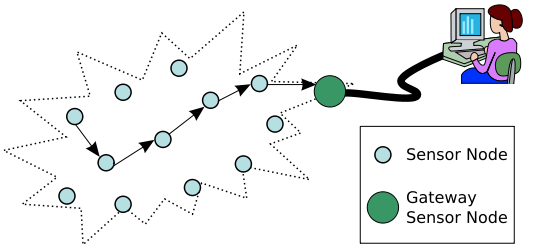
\includegraphics[width=\textwidth]{images/wsn.png}
  \end{column}
  \begin{column}{0.3\textwidth}
   \centering \liuhao{mica2, mica2dot(伯克利)}\\
   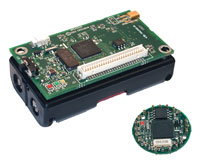
\includegraphics[width=.9\textwidth]{images/mica_family.jpg}\\
   \liuhao{FLOWS3(清华)}\\
   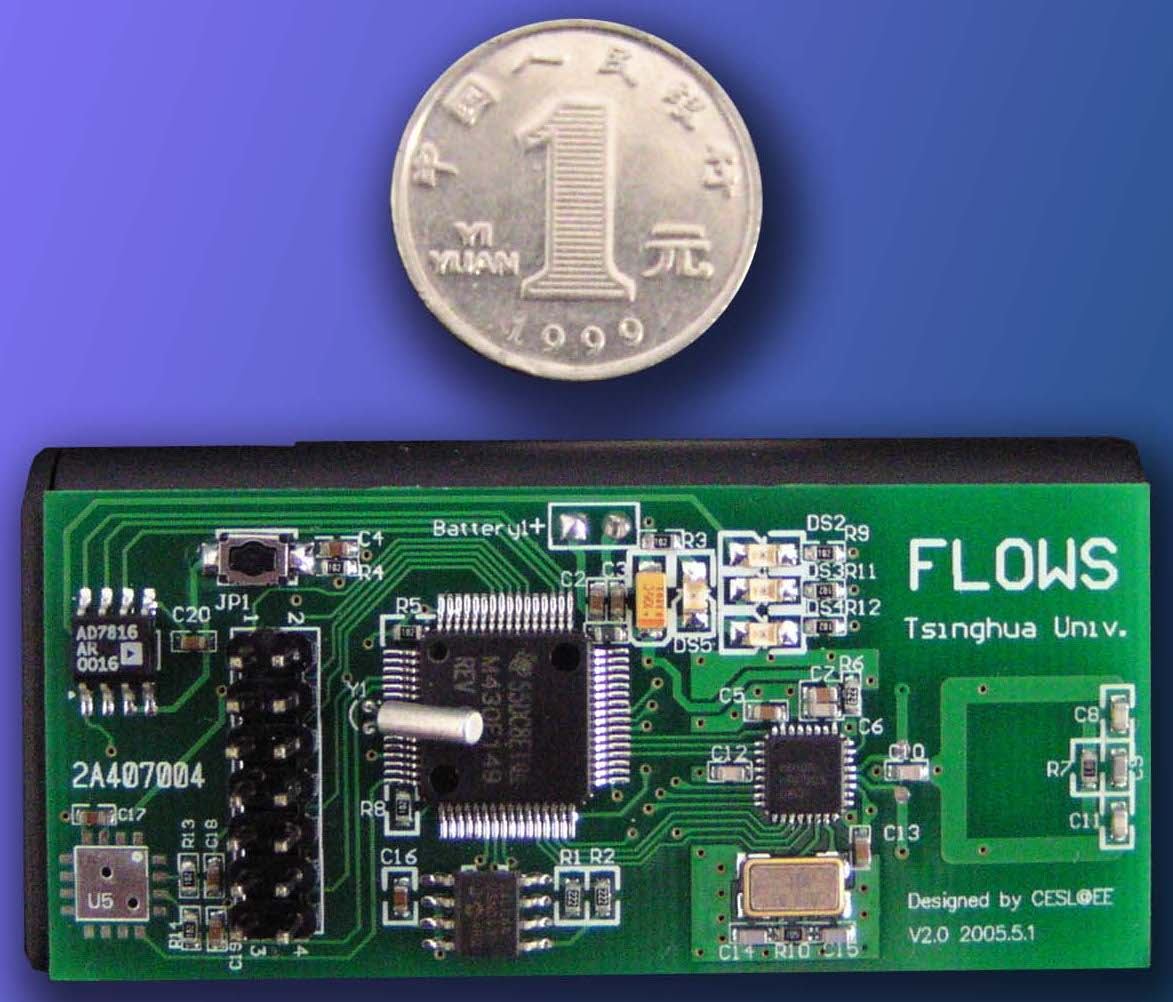
\includegraphics[width=\textwidth]{images/flows3.jpg}
  \end{column}
\end{columns}
\end{frame}

\begin{frame}{WSN~中节点的位置信息}

\textbf{节点的位置信息}是无线传感器网络中的一项重要信息,有着非常广泛的应用:

\begin{columns}
  \begin{column}{0.5\textwidth}
\begin{itemize}
\item 节点定位
\item 目标追踪
\item 数据的识别和关联
\item 得到网络能量分布图
\item 评估节点密度和覆盖范围
\item 指定区域节点的管理和查询
\item 基于地理位置的路由和密钥管理
\end{itemize}
  \end{column}
  \begin{column}{0.5\textwidth}
  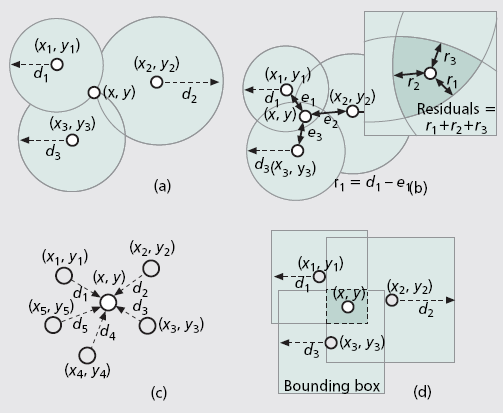
\includegraphics[width=\textwidth]{images/localization.png}
  \end{column}
\end{columns}
\end{frame}

\section{研究现状}

\begin{frame}{大纲}
	\tableofcontents[currentsection]
\end{frame}

\subsection{安全定位算法}

\begin{frame}{WSN~中的安全定位算法}
\begin{itemize}
\item 密码学手段
\begin{itemize}
\item 加密和数据源认证,保证定位消息的安全传输
\item SeRLoc \cite{Lazos2005}, SPINE \cite{Capkun2005, Capkun2006}, ROPE \cite{Lazos2006}, HiRLoc \cite{Lazos2005a}
\end{itemize}
\item 异常行为检测和屏蔽
\begin{itemize}
\item 检测恶意节点的异常行为并屏蔽该节点
\item Liu ICDCS'05 \cite{Liu2005c}, DRBTS \cite{Srinivasan2006}
\end{itemize}
\item 攻击容忍的鲁棒位置算法
\begin{itemize}
\item 使用鲁棒算法消除恶意信息的影响,多使用统计学手段
\item Liu IPSN'05 \cite{Liu2005b}, KPS \cite{Fang2005}, Li IPSN'05 \cite{Li2005a}
\end{itemize}
\item 位置验证技术
\begin{itemize}
\item 对位置算法得到的位置进行验证,判断位置是否异常
\item Echo \cite{Sastry2003}, LAD \cite{Du2006}, \v{C}apkun INFOCOM'06 \cite{Capkun2006a, Capkun2008}
\end{itemize}
\end{itemize}
\end{frame}

\begin{frame}{WSN~中的安全定位算法}
\centerline{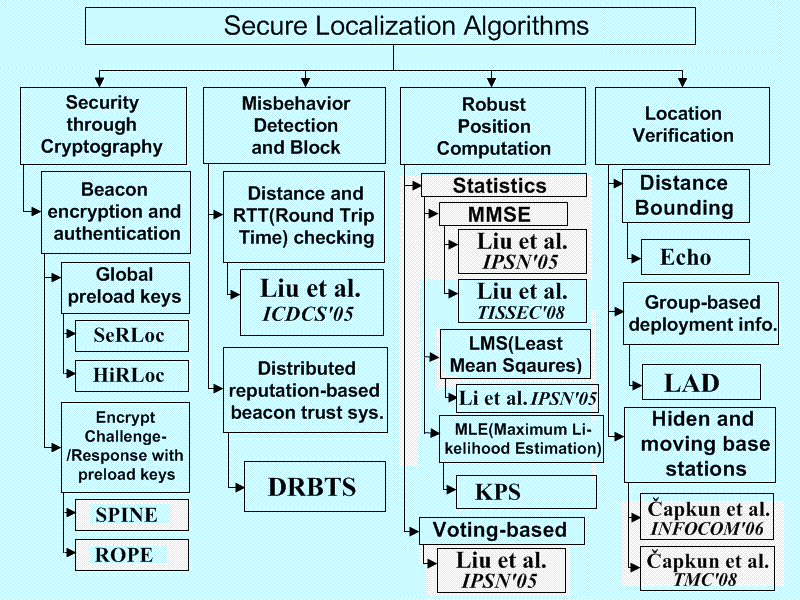
\includegraphics[width=.8\textwidth]{images/wsn_sec_pos.png}}
\end{frame}

\subsection{位置信息的保护和应用}

\begin{frame}{WSN~节点位置信息的保护和应用}

\begin{block}{节点位置信息私密性的保护}
\begin{itemize}
\item 保护节点位置不被敌方获得,例如关键节点位置不被发现
\item 主要采用数据融合、虚假路由、增加虚假流量等方式
\item Gruteser HOTOS'03 \cite{Gruteser2003}, Ozturk SASN'04 \cite{Ozturk2004}, GROW \cite{Xi2006}
\end{itemize}
\end{block}

\bigskip

\begin{block}{位置信息在其它安全算法中的应用}
\begin{itemize}
\item 已知位置能够提供给其它安全算法额外的信息
\item 目前主要的应用是利用部署信息降低密钥分配的复杂度
\item Liu SASN'03 \cite{Liu2003}, Huang SASN'04 \cite{Huang2004}
\end{itemize}
\end{block}
\end{frame}

\section{研究内容和研究方法}

\begin{frame}{大纲}
	\tableofcontents[currentsection]
\end{frame}

\subsection{研究内容}

\begin{frame}{研究内容}
\begin{itemize}
\item 探索更适合~WSN~的简单的安全定位方法
\begin{itemize}
\item \xiaowuhao{目前的安全定位方法要求定位者节点具有更强的硬件(GPS,定向天线等),应用上依然有困难。}
\end{itemize}
\item 寻找更鲁棒的安全定位算法
\begin{itemize}
\item \xiaowuhao{异常节点的识别和排除主要使用统计学方法,我们希望找到使定位算法能够更鲁棒的方法。}
\end{itemize}
\item 将安全定位与其它安全方案相结合
\begin{itemize}
\item \xiaowuhao{考虑到安全定位算法与其它安全方案可以共享一些信息和模块,将它们结合一起考虑,希望会发现更优的算法。}
\end{itemize}
\item 设计开销与隐私保护更均衡的位置私密性保护方案
\begin{itemize}
\item \xiaowuhao{希望能降低在网络中使用虚假路由或者引入虚假流量来迷惑敌手引入的通信开销。}
\end{itemize}
\end{itemize}
\end{frame}

\subsection{研究方法}
\begin{frame}{研究方法}
\begin{itemize}
\item 综合评估现有安全定位方法的特点与不足
\begin{itemize}
\item \xiaowuhao{从抵御的攻击类型、硬件要求、定位精确度、算法复杂度、通信开销、可扩展性等几个方面对它们进行比较分析。}
\end{itemize}
\item 对基于统计的定位算法进行详细研究
\begin{itemize}
\item \xiaowuhao{探索每个统计模型适用范围和对错误数据的容忍程度,寻找更健壮的统计模型。}
\end{itemize}
\item 比较安全定位与其它方案,找出可共同利用的信息和模块
\begin{itemize}
\item \xiaowuhao{研究安全定位与密钥管理、数据融合、安全路由等安全方案,从算法、协议等处寻找可共同利用的部分。}
\end{itemize}
\item 提出新的安全定位方案并进行仿真实验
\begin{itemize}
\item \xiaowuhao{以提高定位算法的安全性和健壮性、降低算法和协议的复杂度为目的,构造新的安全定位方案并进行仿真。}
\end{itemize}
\item 进一步探索位置信息的私密性保护和应用
\begin{itemize}
\item \xiaowuhao{分析已有方案中各部分保护效果和开销,寻找减轻通信开销的替代方法;评价位置信息能否使其它方案产生更优的结果。}
\end{itemize}
\end{itemize}
\end{frame}

\section{研究工作进度安排}

\begin{frame}{研究工作进度安排}
\begin{itemize}
\item 2008年09月-2008年12月:调研~WSN~节点位置安全相关文献,总结攻击形式和安全技术的发展状况,完成开题报告。
\item 2009年01月-2009年09月:完成~WSN~安全定位算法的模型设计、理论论证和仿真比较工作,基于研究成果,撰写一到两篇论文。
\item 2009年10月-2009年12月:进一步完善改进设计方案,准备中期答辩。
\item 2010年01月-2010年06月:总结归纳研究成果,撰写毕业论文。
\end{itemize}

\end{frame}

\section{参考文献}

\begin{frame}[allowframebreaks]{参考文献}
\tiny
\bibliographystyle{IEEEtran}
\bibliography{IEEEabrv,wsn}
\end{frame}

\section*{Q\&A}

\begin{frame}{Q\&A}
\begin{block}{}
\centerline{\chuhao{Q\&A}}
\end{block}
\end{frame}
\end{CJK*}
\end{document}
